%% Version 4.3.1, 19 May 2014
%
%%%%%%%%%%%%%%%%%%%%%%%%%%%%%%%%%%%%%%%%%%%%%%%%%%%%%%%%%%%%%%%%%%%%%%
% Template.tex --  LaTeX-based template for submissions to the 
% American Meteorological Society
%
% Template developed by Amy Hendrickson, 2013, TeXnology Inc., 
% amyh@texnology.com, http://www.texnology.com
% following earlier work by Brian Papa, American Meteorological Society
%
% Email questions to latex@ametsoc.org.
%
%%%%%%%%%%%%%%%%%%%%%%%%%%%%%%%%%%%%%%%%%%%%%%%%%%%%%%%%%%%%%%%%%%%%%
% PREAMBLE
%%%%%%%%%%%%%%%%%%%%%%%%%%%%%%%%%%%%%%%%%%%%%%%%%%%%%%%%%%%%%%%%%%%%%

%% Start with one of the following:
% DOUBLE-SPACED VERSION FOR SUBMISSION TO THE AMS
%\documentclass{ametsoc}

% TWO-COLUMN JOURNAL PAGE LAYOUT---FOR AUTHOR USE ONLY
\documentclass[twocol]{ametsoc}

%%%%%%%%%%%%%%%%%%%%%%%%%%%%%%%%
%%% To be entered only if twocol option is used

\journal{jcli}

%  Please choose a journal abbreviation to use above from the following list:
% 
%   jamc     (Journal of Applied Meteorology and Climatology)
%   jtech     (Journal of Atmospheric and Oceanic Technology)
%   jhm      (Journal of Hydrometeorology)
%   jpo     (Journal of Physical Oceanography)
%   jcli      (Journal of Climate)
%   mwr      (Monthly Weather Review)
%   wcas      (Weather, Climate, and Society)
%   waf       (Weather and Forecasting)
%   bams (Bulletin of the American Meteorological Society)
%   ei    (Earth Interactions)

%%%%%%%%%%%%%%%%%%%%%%%%%%%%%%%%
%Citations should be of the form ``author year''  not ``author, year''
\bibpunct{(}{)}{;}{a}{}{,}

%%%%%%%%%%%%%%%%%%%%%%%%%%%%%%%%

%%% To be entered by author:

%% May use \\ to break lines in title:

%\title{Atmospheric response to simulated historical sea ice loss}
\title{Isolating the impact of human-induced Arctic sea ice loss on the atmosphere}

%%% Enter authors' names, as you see in this example:
%%% Use \correspondingauthor{} and \thanks{Current Affiliation:...}
%%% immediately following the appropriate author.
%%%
%%% Note that the \correspondingauthor{} command is NECESSARY.
%%% The \thanks{} commands are OPTIONAL.

    %\authors{Author One\correspondingauthor{Author One, 
    % American Meteorological Society, 
    % 45 Beacon St., Boston, MA 02108.}
% and Author Two\thanks{Current affiliation: American Meteorological Society, 
    % 45 Beacon St., Boston, MA 02108.}}

\authors{Kelly E. McCusker\correspondingauthor{School of Earth and Ocean Sciences, University of Victoria, Victoria, BC, Canada.}}

%% Follow this form:
    % \affiliation{American Meteorological Society, 
    % Boston, Massachusetts.}

\affiliation{University of Victoria,
                      Victoria, British Columbia}

%% Follow this form:
    %\email{latex@ametsoc.org}

\email{kemccusk@uvic.ca}

%% If appropriate, add additional authors, different affiliations:
    %\extraauthor{Extra Author}
    %\extraaffil{Affiliation, City, State/Province, Country}

\extraauthor{John C. Fyfe}
%\extraaffil{}

%% May repeat for a additional authors/affiliations:

\extraauthor{Michael Sigmond}
\extraaffil{University of Victoria,
                      Victoria, British Columbia}



%%%%%%%%%%%%%%%%%%%%%%%%%%%%%%%%%%%%%%%%%%%%%%%%%%%%%%%%%%%%%%%%%%%%%
% ABSTRACT
%
% Enter your Abstract here

%\abstract{Changes in Arctic sea ice play an important role in modulating surface fluxes of heat and moisture, and therefore local near-surface temperatures and precipitation. Whether or not historical sea-ice retreat has had a marked influence on weather patterns, particularly outside the local region, remains an open and important question. Here the effect historical sea-ice loss has on the atmosphere is isolated by prescribing observed sea-ice concentrations and local sea surface temperatures in an atmosphere model. A suite of 120-year simulations is carried out to temper natural variability. We find that observed boundary conditions produce a lowering of Arctic sea level pressure in Autumn that is robust and consistent with other studies, but no clear signal in patterns of variability emerge. Furthermore, the response to observed sea-ice changes is compared to a suite of simulations in which boundary conditions are obtained from an ensemble of historical simulations from a coupled global climate model. We find that whereas near-surface temperature responds in accordance with the amount of sea ice loss --- more loss yields larger warming --- sea-level pressure and geopotential heights remain slave to natural variability. Individual ensemble members have regions and seasons of statistically significant circulation changes in response to sea-ice loss, however those regions and seasons are not robust across ensemble members. Thus, it is likely that 1. historical sea-ice loss played a minimal role in setting circulation trends and 2. any detectable effect sea-ice loss had is due to @@ Thus, caution must be taken when interpreting even long time-slice simulations  @@. Notably, the observed forcing produces a response that is outside the bounds of the } % Harder to tease out is how changes in sea ice influence local and remote circulation. % natural variability for determining both the sea-ice forcing pattern and the response to sea-ice loss by prescribing an ensemble of boundary conditions obtained from a coupled model's ensemble of historical simulations. %...@@. The importance of the pattern of sea-ice loss is further examined by prescribing a suite of boundary conditions obtained from a coupled model's ensemble of historical simulations. 


%Isolating the Impact of human-induced Arctic Sea Ice Loss on the Atmosphere

\abstract{Changes in Arctic sea ice play an important role in modulating surface fluxes of heat and moisture, and therefore local near-surface temperatures and precipitation. Whether or not historical sea-ice retreat has had a marked influence on remote climatic changes remains an open and important question. Here the effects of historical sea-ice loss on the atmosphere are isolated by prescribing Arctic sea ice loss from two different observational datasets to an atmosphere-only model. In addition, we prescribe to the atmosphere-only model sea ice loss patterns simulated by an ensemble of historical simulations with the corresponding coupled model. These simulations allow for the separation of the climate effects of forced (human-induced) sea ice loss and the climate effects of (random) sea ice changes induced by internal variability. We find that all scenarios exhibit a robust, shallow Arctic warming, a tendency for lower Arctic sea level pressure, and higher geopotential heights aloft in Autumn and Winter. However, the pattern and magnitude of circulation change outside the Arctic and at upper levels varies widely across simulations. We suggest that internal variability in the sea ice anomaly pattern itself is an important driver in determining midlatitude changes to observed Arctic sea ice loss.
} % Slightly modified AGU Abstract


\begin{document}

%% Necessary!
\maketitle


%%%%%%%%%%%%%%%%%%%%%%%%%%%%%%%%%%%%%%%%%%%%%%%%%%%%%%%%%%%%%%%%%%%%%
% MAIN BODY OF PAPER
%%%%%%%%%%%%%%%%%%%%%%%%%%%%%%%%%%%%%%%%%%%%%%%%%%%%%%%%%%%%%%%%%%%%%
%

%% In all cases, if there is only one entry of this type within
%% the higher level heading, use the star form: 
%%
% \section{Section title}
% \subsection*{subsection}
% text...
% \section{Section title}

%vs

% \section{Section title}
% \subsection{subsection one}
% text...
% \subsection{subsection two}
% \section{Section title}

%%%
% \section{First primary heading}

% \subsection{First secondary heading}

% \subsubsection{First tertiary heading}

% \paragraph{First quaternary heading}

\section{Introduction}

Arctic sea ice has made a dramatic transformation over the late 20th and early 21st century due in large part to increasing greenhouse gas concentrations. Sea ice concentrations are at record lows since at least 1900@@, multi-year ice is declining, and the ice overall is thinner (2012 record low Zhang et al 2013, Parkinson and Comiso 2013). These changes are both caused by greenhouse warming and help to amplify greenhouse warming in the high northern latitudes such that the Arctic is warming at a rate 2-3 times as large as the rest of the globe (@@). The reduction in sea-ice area unmasks the ocean below, allowing its darker waters to collect heat in sunlit months which it subsequently releases to the relatively colder atmosphere in winter months. The question remains as to how large of an influence this loss of sea ice has on the atmosphere, both locally and remotely. %  increasing heat flux from the warmer waters to the relatively cold atmosphere in winter months. 

Studies in which sea ice is artificially reduced by prescribing sea ice and sea surface temperature (SST) conditions in an atmosphere model all agree that when sea ice area or extent decreases, turbulent heat fluxes increase into the atmosphere, surface air temperature increases, and generally local sea level pressure (SLP) is reduced (@@cite all the things). Considerable disagreement exists, however, when attempting to determine how the atmospheric circulation responds, especially non-locally. 

Much study has 

An important question

Lit review here. Singarayer et al. 2005 compares responses to 3 observational sea ice datasets.

Studies that implement time-slice simulations with similar prescribed boundary conditions from comparable time periods 

It is worth noting that the vast majority of previous studies investigating the response of the atmosphere to changes in sea ice have been accomplished under two model lineages: National Center for Atmospheric Research Community atmosphere models, and atmosphere models developed by the Hadley Centre. Thus, a primary motivation for undertaking this study is to add a much-needed third data point from the Canadian Centre for Climate Modelling and Analysis atmosphere model to the growing literature about the influence of sea ice loss on the atmosphere. Moreover, 

\section{Model and simulations}

To isolate the effect of sea ice on the atmosphere, we use the Canadian Centre for Climate Modelling and Analysis fourth-generation atmosphere general circulation model (CanAM4) with prescribed surface boundary conditions and a freely evolving atmosphere. The model is run at T63 horizontal resolution with 37 vertical levels from the surface up to 1hPa. Further model details can be found in @@cite. We execute a suite of 121-year time-slice simulations and analyze the last 120 years in the results. Each simulation is prescribed with an annually repeating seasonal cycle of sea-ice concentration (SIC), sea-ice thickness (SIT), and sea surface temperatures (SST) as described below. The greenhouse gas, tropospheric aerosol, and solar levels are set to 1984 conditions for all simulations. In this way, any resulting changes in climate can be attributed to changes in the prescribed surface forcing alone.

% boundary conditions
\subsection{Boundary conditions}
\subsubsection{Historical observations}

In order to investigate the effect of observed sea ice loss on the atmosphere, we utilize two gridded data products of observed sea ice concentration. First, gridded sea-ice concentration and sea surface temperature data prepared by the Hadley Centre (Hadley Centre sea ice and SST dataset, version 1.1; HadISST1.1 @@cite) are used as boundary conditions to CanAM4. Second, sea-ice concentrations from the National Snow and Ice Data Center (NSIDC) and constructed using the Bootstrap algorithm (@@) are utilized (@@cite). HadISST1.1 has previously been used as surface boundary conditions for the IPCC Atmosphere Model Intercomparison Project (AMIP), as well as in previous work attempting to tease out the isolated effect of sea ice loss on the atmosphere (cite@@). However, because HadISST1.1 has been shown to underestimate the trend in sea ice loss (cite@@), we also utilize NSIDC sea ice concentration coupled with HadISST1.1 SSTs (adjusted for consistency with NSIDC SIC) as boundary conditions. An earlier version of the NSIDC bootstrap sea ice concentration dataset has been evaluated and shown to @@ (Singarayer et al. 2005). 

The effect of sea ice loss is examined over the satellite era, from 1979 onwards, when the observations are most reliable and the changes in sea ice are greatest. The control simulation is run for 121 years with 1979-1989 monthly mean annually-repeating climatologies of HadISST1.1 SIC and SST (\textbf{HADctl}). Similarly, a control simulation is run with a 1979-1989 monthly mean annually-repeating climatology of NSIDC SIC (\textbf{NSIDCctl}). Because NSIDC data are only sea ice concentrations, we pair HadISST1.1 SST with NSIDC SIC in \textbf{NSIDCctl}, with SST adjusted so that grid cells without sea ice in NSIDC but with sea ice in HadISST1.1 are set to the freezing temperature of seawater (271.2 K). The sea ice thickness boundary condition used in the HAD and NSIDC set of simulations is a climatology of sea ice thickness obtained from a previous CanAM model version (@@Merryfield). The thickness is held constant at the control (1979-1989) thickness for all simulations, except where SIC disappears, where it is set to zero. We have adjusted the thickness to be consistent with the HadISST1.1 sea ice concentration, and the NSIDC sea ice concentration by setting SIT to zero when SIC is zero. Boundary conditions in Autumn for HAD are shown as differences (HADpt minus HADctl) in Figures \ref{fig:fig1}a-c. For simplicity, we leave out NSIDC boundary condition patterns as they are very similar to HAD in Autumn, however seasonal cycles for all simulations are shown in Figure \ref{fig:fig2}. Note that SST anomalies are only shown where SIC is less than 0.15 in HADctl, where the model considers the grid cell to be open water (check with ML@@).

%Perturbation simulations are run with 2002-2011 monthly mean annually-repeating climatologies of HadISST1.1 SIC in \textbf{hadPT}, and NSIDC SIC in \textbf{nsidcPT}. The SST boundary condition in the perturbed simulations is the same as their respective control simulations (1979-1989 climatology), except where sea ice concentration has decreased by at least 10\%, in which case the SST is set to the 2002-2011 climatology. In this way, only changes in SST directly attributed to changes in sea ice are incorporated. This method has been previously used in Screen@@, Peings and Magnusdottir@@. 


%Autumn boundary condition anomaly patterns for HadISST are shown in Figure \ref{fig:fig1} with the seasonal cycle of all simulations shown in Figure \ref{fig:fig2}.

%Perturbed sea ice conditions representing sea ice loss are simulated by running CanAM4 with 2002-2011 climatologies of SIC

 and 2002-2011 monthly mean climatologies of SIC and SST as the perturbed (low ice) simulation, \textbf{HADpt}. These monthly climatologies are used as repeating boundary conditions in CanAM4 for 121 years, as described next. Because the boundary conditions are annually repeating and the atmosphere has a short memory on the timescale of days (@@), each year can be considered an independent realization of the state of the atmosphere. Thus, after throwing out the first year for spin-up, the ensemble size, N, of each simulation is 120.  % . While HadISST1.1 has some known biases @@cite, it is somewhat of an "industry standard" and has been used as boundary conditions for IPCC Atmosphere Model Intercomparison Projects (AMIP) as well as previous work attempting to tease out the effect of sea ice loss on the atmosphere @@cite. 

%The control simulation with observed HadISST boundary conditions is forced with a repeating HadISST1.1 1979-1989 monthly climatology of SIC and SST and is called \textbf{hadCTL}. hadCTL sea ice thickness boundary condition data is obtained from the output of a previous CanAM model version (@@Merryfield). The perturbation simulation, called \textbf{hadPT}, is forced with a repeating HadISST1.1 2002-2011 monthly climatology of SIC, and 1979-1989 SST everywhere except where SIC declines by 10\% or more, in which case SST is the 2002-2011 climatology. In this way, only changes in SST directly attributed to changes in sea ice are incorporated. This method has been previously used in Screen@@, Peings and Magnusdottir@@. The hadPT SIT boundary condition is the same as for hadCTL, except that where SIC disappears, SIT is set to zero. We discuss the relative importance of including changes in both local SST and sea-ice thickness in Section @@.

Additionally, to examine the importance of biases in the HadISST boundary conditions on the resulting climate response, we utilize gridded sea-ice concentrations from the National Snow and Ice Data Center (NSIDC)

[Describe other sims here]

Unless otherwise noted, results will be presented as anomalies from the 120-year average of the respective control simulation, and will be referred to as 'HAD' and 'nsidc'. When looked at in this way, the forcing is effectively the anomaly patterns of sea-ice concentration, thickness, and SST. 
 
\subsubsection{Historical model simulations}

 We contrast results obtained from forcing with observed sea ice and SST conditions with those 

 obtained from  and historical simulations of the second generation Canadian Earth System Model (CanESM2).
% HadISST1.1 ref: http://www.esrl.noaa.gov/psd/data/gridded/data.hadsst.html (not sure it was obtained here...)
% Rayner, N. A.; Parker, D. E.; Horton, E. B.; Folland, C. K.; Alexander, L. V.; Rowell, D. P.; Kent, E. C.; Kaplan, A. (2003) Global analyses of sea surface temperature, sea ice, and night marine air temperature since the late nineteenth century J. Geophys. Res.Vol. 108, No. D14, 4407 10.1029/2002JD002670 

%, 'can', 'can_e[1-5]', 'can_e4nosit', 'can_nosit', and 'can_nosst'. 

\begin{table*}[t]
\caption{Model simulation details. Diff name is used when describing the results as anomalies; e.g. HAD means Hadpt - Hadctl. The sensitivity simulations are listed at the bottom of the table and their corresponding control simulation is CANctl1. All simulations have a constant annually-repeating set of boundary conditions and are run for 121 years with the first year disregarded for analysis.}\label{simstbl}
\begin{center}
\begin{tabular}{llcccccc}
\hline\hline
Diff Name & Sim & SIC & SIT & SST & BC Source & Notes\\
\hline
HAD &  HADctl   & 1979-89 & 1979-89 & 1979-89 & HadISST1.1 \\
         & HADpt &   2002-11 & 1979-89* & 2002-11 & HadISST1.1 & *SIT set to 0 where SIC 0 \\
            &                 &               &                &                &                     &     and @@\\
 NSIDC & NSIDCctl  &1979-89 & 1979-89 & 1979-89 & NSIDC \\
             & NSIDCpt &   2002-11 & 1979-89* & 2002-11 & NSIDC & *SIT set to 0 where SIC 0 \\
               &              &                &                 &               &              &   and @@\\
 TOT[1-5] & CANctlBC[1-5] & 1979-89 & 1979-89 & 1979-89  & CanESM2 historical ensemble members 1-5  & \\
                & CANptBC[1-5] &   2002-12 & 2002-12 & 2002-12 &  CanESM2 historical ensemble members 1-5  & \\
 \\
 ANTH[1-5] &  CANctl[1-5] &    1979-89 & 1979-89 & 1979-89 & CanESM2 historical ensemble average & 1-5 have varied initial conditions \\
                   & CANpt[1-5] & 2002-12 & 2002-12 & 2002-12 &  CanESM2 historical ensemble average &  1-5 have varied initial conditions \\
  \hline
 \hline
 ANTH1nosit   & CANpt1nosit &     2002-12 & 1979-89* & 2002-12 &  CanESM2 historical ensemble, & *SIT set to 0 where SIC 0. \\
                       &                       &                 &                  &              &       average, member 1             & \\
ANTH1nosst  &  CANpt1nosst &      2002-12 & 2002-12 & 1979-89 &  CanESM2 historical ensemble  & \\
                        &                       &                 &                  &              &       average, member 1             & \\
TOT4nosit   &  CANptBC4nosit  &    2002-12 & 1979-89* & 2002-12 &  CanESM2 historical ensemble member 4 & *SIT set to 0 where SIC 0. \\
\hline
\end{tabular}
\end{center}
\end{table*}


\section{Results}

We start by considering the climate response to HadISST1.1 sea ice loss between 2002-2011 and 1979-1989 by subtracting the 120-year average of HADct from the 120-year average of HADpt, which will be referred to simply as \textit{HAD}. Figure \ref{fig:fig1}a shows the pattern of ice loss in Autumn (SON) when the loss is greatest, and Figure \ref{fig:fig2}a shows the seasonal cycle of Arctic sea ice area anomalies. HadISST1.1 has the greatest loss of ice in October and very little sea ice loss through late winter and spring. Accordingly, surface air temperature in \textit{HAD} area-averaged over the polar cap (north of 70$^\circ$N) warms only a nominal amount from about January to August, but shows average warming of almost 3$^\circ$C in November. The slight lag in maximum surface warming compared to maximum sea ice loss can be understood by considering the timing of maximum surface fluxes to the atmosphere. Figure \ref{fig:fig2}b shows how the net surface flux is greatest in October and November whereas sea ice reductions are greatest in September and October. This feature has been previously noted (cite@@ Deser2010, Screen2013, PandM 2014...)) and is primarily due to the optimal combination of newly opened waters from the loss of sea ice plus the climatologically colder overlying air drawing more heat out of the newly opened waters. 

The effect of sea ice loss on the atmosphere is communicated by these changes in surface flux. The resulting thermal response is a broad, uniform warming over the polar cap and northern-most land surfaces particularly in Autumn (Figure @@). Northern Canada and Hudson Bay region, the northeast United States and northern Eurasia north of about 60$^\circ$N experience statistically significant warming upwards of 3$^\circ$C, reaching even 5$^\circ$C in some places. Winter is also warmer by up to 5$^\circ$C in some locations, however there are regions of cooling over the highest latitudes near sea ice growth in the HadISST1.1 dataset, somewhat balancing out polar cap averaging.

 A statistically significant zonal mean warming remains relatively local and shallow, warming in altitude up to about 700 hPa and south to about 55$^\circ$N in SON and DJF (@@add Vert fig).

The thermal response to HadISST1.1 observed sea ice loss is consistent with previous studies that have similar experimental designs but utilize different AGCMs (@@cite).

Previous studies have prescribed boundary conditions derived from


\subsection{Role of internal variability}
% "area-weigted spatial correlations between pairs of panels" -- from Baldwin and Thompson 2009
Our experimental design allows a distinction to be made between the response to the human-induced (forced) sea ice anomaly and that due to historical sea ice change caused by internal variability. Because CAN is forced with an average sea ice anomaly pattern (the average of 5 historical ensemble members) and has a large ensemble size of 120 per simulation (CANctl and CANpt), we assume that the climate response of CAN (CANpt minus CANctl) is the response to human-induced sea ice loss. Later we will discuss the validity of this assumption. Similarly, the climate response of individual ensemble members (E1-5), each forced with the human-induced pattern plus some amount of internal variability, represents the response to both human-induced and chaos-induced sea ice change. To gauge the level of influence internal variability has on the sea ice anomaly pattern, we calculate an area-weighted spatial correlation between the forced anomly pattern (CAN) and each individual ensemble member's sea ice anomaly pattern for each season, using all grid cells greater than 60$^\circ$N. 

The correlations are a measure of the contribution of anthropogenic forcing to the pattern, the residual of which represents the contribution of internal variability. A correlation of 1 would indicate that the ensemble member sea ice anomaly pattern is identical to the forced pattern. Thus, correlations near 1 indicate a greater contribution from anthropogenic forcing to the individual ensemble member pattern. Conversely, correlations near zero indicate almost no match to the forced pattern and thus an almost total contribution from internal variability. The gray bars in Figure \ref{fig:fig4}a show the mean and spread of spatial pattern correlations between E1-5 and CAN SIC anomaly patterns for each season. The largest mean correlation ($>$0.9) occurs in Autumn, when the most sea ice loss occurs, and also exhibits the least uncertainty between ensemble members (Figure \ref{fig:fig4}a). By this measure, almost all of the SIC anomaly pattern in Autumn is human-induced (86\%, calculated as 100 multiplied by the average of the squared individual pattern correlations; Figure \ref{fig:fig4}a). Spring and Summer SIC anomaly patterns contain a greater contribution from internal variability (the residual of 56\% and 62\%, respectively) as well as display a larger spread across ensemble members. Nevertheless, correlations in all seasons and ensemble members are large and easily statistically significant at the 95\% level, with an annual mean pattern correlation greater than 0.7 for all E1-5, and an annual mean contribution from the anthropogenic pattern of 68\%.
% then the resulting value (r2, the coefficient of determination) will represent the proportion of common variation in the two variables (i.e., the "strength" or "magnitude" of the relationship)  http://www.statsoft.com/Textbook/Basic-Statistics#Correlations

Recall that the sea ice anomaly patterns are prescribed boundary conditions in our simulations and so these correlations represent the contribution of anthropogenically forced sea ice changes to the 'forcing' in our simulations (see schematic?@@). We can make the same calculation between the response patterns as well, to identify the degree to which the response to a representation of sea ice loss (E1-5) matches the response to forced sea ice loss (CAN). In other words, how important is internal variability in the sea ice loss pattern for determining the climate response to sea ice loss? 

Gray bars in Figure \ref{fig:fig4}b and \ref{fig:fig4}c show seasonal spatial correlations between the response patterns of E1-5 and CAN for SAT (Figure \ref{fig:fig4}b) and SLP (Figure \ref{fig:fig4}c) north of 60$^\circ$N. As with SIC, the SAT response pattern is most closely tied to the human-induced pattern in Autumn, when the largest SIC reduction and resultant surface warming occurs (Figure \ref{fig:fig2}a and c). Moreover, the uncertainty around the high correlations in both Autumn and Winter is small. Thus, in Autumn and Winter, internal variability in the SAT response is overwhelmed by the human-induced SAT response. However, in Spring and especially Summer, internal variability is the primary factor in determining the SAT response pattern. Internal variability is also the key factor in the SLP response, year-round. The highest contribution from the human-induced forcing occurs in Winter, but there is considerable spread in the correlations, the lowest of which are not statistically significant. The only season in which all correlations are positive, statistically significant, and have a relatively small uncertainty range is again Autumn. In this season, as with SIC and SAT, the response tends to be largest (particularly in November; Figure \ref{fig:fig2}d) exhibiting thermal lows over the polar cap.

Thus, internal variability plays a smaller role in setting the SIC pattern and the response to that SIC pattern in Autumn, when the forcing (sea ice loss) is largest. This is particularly true for thermodynamic fields (SAT), and far less so for dynamical fields (SLP). These results are consistent with the idea that circulation-related fields are much more influenced by internal variability than thermodynamic fields (Screen et al. 2013). @@implication@@ Here we have taken advantage of the fact that the forced pattern (CAN) is 'known'. In reality, there is but one realization of sea ice evolution, which is influenced by anthropogenic forcing as well as chaotic atmospheric motions (and oceanic to some extent). How different might the response to sea ice loss be under a different representation of sea ice evolution?

@@@
Of course, in reality, there is but one realization of sea ice change, which includes human-induced forcing as well as internal variability. How different might the response to sea ice loss be under a different representation of sea ice change? We can use our ensemble of simulations (E1-5) to help understand the importance of the contribution from internal variability by assuming that one ensemble member represents "observations", while the rest of the ensemble members represent other potential outcomes due to internal variability. Correlating "observations" with each of the other potential outcomes and then repeating for each of the ensemble members reveals how similar (indicating less internal variability) or different (indicating more internal variability) other potential realities may have been compared to the "observations".  The number of correlation combinations is the factorial of the ensemble size; $N! = 10$, which are shown in Figure \ref{fig:fig4}@@. The resulting correlations follow similar relationships to those in Figure \ref{fig:fig4}, but are lower, and have much greater uncertainty. Some ensemble members sea ice anomaly patterns match "observations" quite well, especially in Autumn, however correlations drop and uncertainty increases significantly in other seasons, especially Spring and Summer. Note that while Winter exhibits some high correlations, it also has a very high spread in correlations

In fact, only 36\% of the Winter sea ice anomaly patterns 

This implies that i. internal variability is least important in 

\begin{enumerate}
\item Observational BCs
	\begin{itemize}
	\item a. Describe HadISST results compared to previous studies.
    	\item b. NSIDC results compared to previous studies.
	\item c. HadISST compared to NSIDC. importance of correct trend (?). importance of pattern (?). transition to diff pattern from CanESM

	\item Figures:
		\begin{itemize}
		\item F1. Sea cycle of surface flux, SIC, SST (have mod runs too?)
	 	\item F2. Fall + Winter NH SAT, SLP, Z500? for Had and NSIDC	
		\item F3. Vertical Fall + Winter T, Z, U for Had and NSIDC	
		\end{itemize}
	\end{itemize}

\item Model BCs
	\begin{itemize}
	\item a. Compare HadISST/NSIDC to averageBC simulation, PERT3??
	\item b. Model BCs with and without SST change, SIT change (sensitivity runs, short section?)
	
	\item Figures:
		\begin{itemize}
		\item F4. Fall + Winter NH SAT, SLP, Z500? for PERT1, PERT2, PERT3? (4x3)
		\item F5. Vertical Fall + Winter T, Z, U for sensitivity runs (OR zonalmean with all sims including E runs?)  
                       \end{itemize}
	
	
	\item c. Put averageBC, Had/NSIDC in context using E1-5 and mean of E's
		\begin{itemize}
		\item How robust is each pattern of response? (pattern corr) How much does pattern of forcing matter?
		\item spread of E members is still smaller than uncertainty in time
		\item HadISST out of bounds of our model --> responses are different, so models may not be capturing proper historical circ response (?)
		\item Robust signal in N Atlantic DJF across almost all members --> what is this and what does it mean? 
		\end{itemize}

	\item d. Near-future confirms DJF Z signal

	\end{itemize}

\end{enumerate}

\section{Discussion and Conclusions}

Thus, recent changes in weather and circulation cannot be definitively attributed to sea ice loss. Rather changes outside the Arctic are more likely to be due to greenhouse gas increases, changes in aerosol concentrations, and/or the most likely culprit: internal variability.

\begin{figure}[t]
  \noindent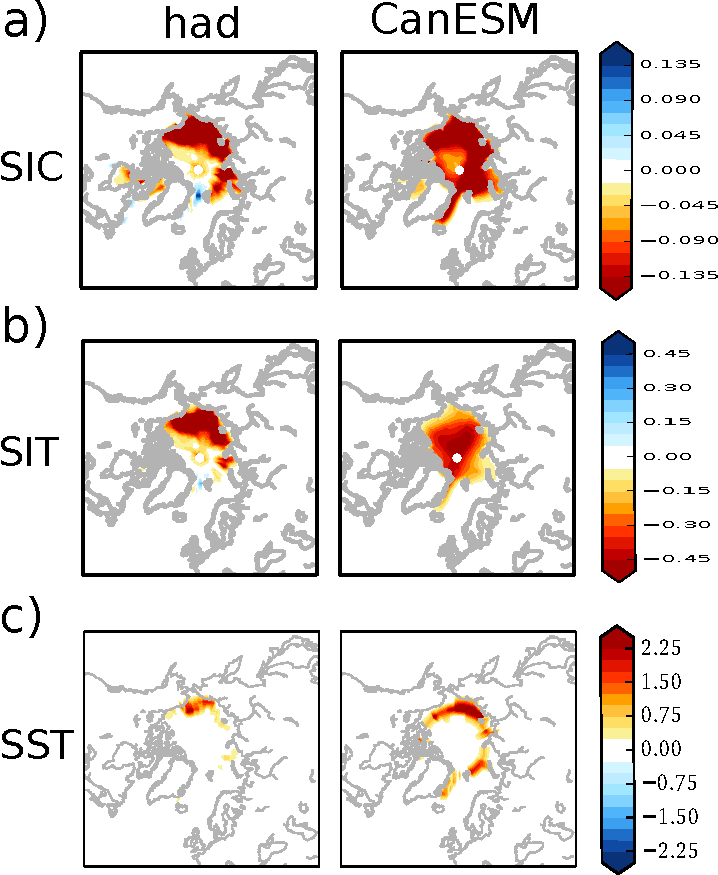
\includegraphics[width=19pc,angle=0]{oneseasBCsnonsidc.pdf}\\
  \caption{a) The difference in mean sea ice concentration (\%) prescribed as boundary conditions in HADctl (1979-89) and HADpt (2002-2011; left column) in Autumn (SON). The right column is as the left column but shows the difference between canPT and canCTL, respectively. b) and c) are as a) but show SIT and SST, respectively.
}\label{fig:fig1}
\end{figure}


\begin{figure}[t]
  \noindent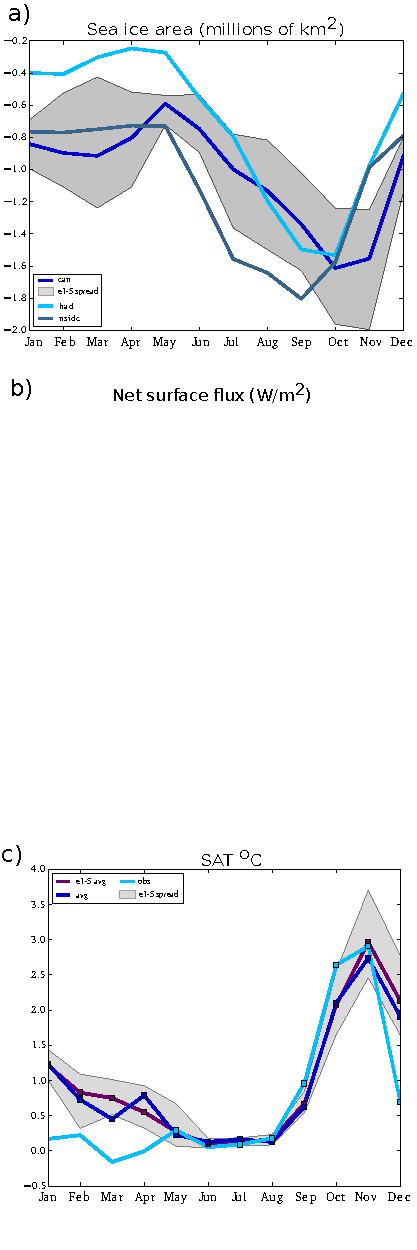
\includegraphics[width=15pc,angle=0]{seacycles.pdf}\\
  \caption{Seasonal cycle of a.) Arctic sea ice area anomaly (10$^6$ km$^2$) for HAD (light blue), NSIDC (gray blue), CAN (dark blue), and ENS (magenta; exactly the same as CAN for sea ice area, by design). Gray shading indicates the range of sea ice area anomalies in individual ensemble members. b.) is as a) but for net surface flux anomaly averaged north of 40$^\circ$N where sea ice concentration $>$ 10\%, c.) is as a) but for surface air temperature anomaly averaged north of 70$^\circ$N, and d.) is as a) but for sea level pressure averaged north of 70$^\circ$N. Squares in b), c), and d) indicate a statistically significant anomaly at the 95\% level using a two-sided student's T test.
}\label{fig:fig2}
\end{figure}

\begin{figure}[t]
  \noindent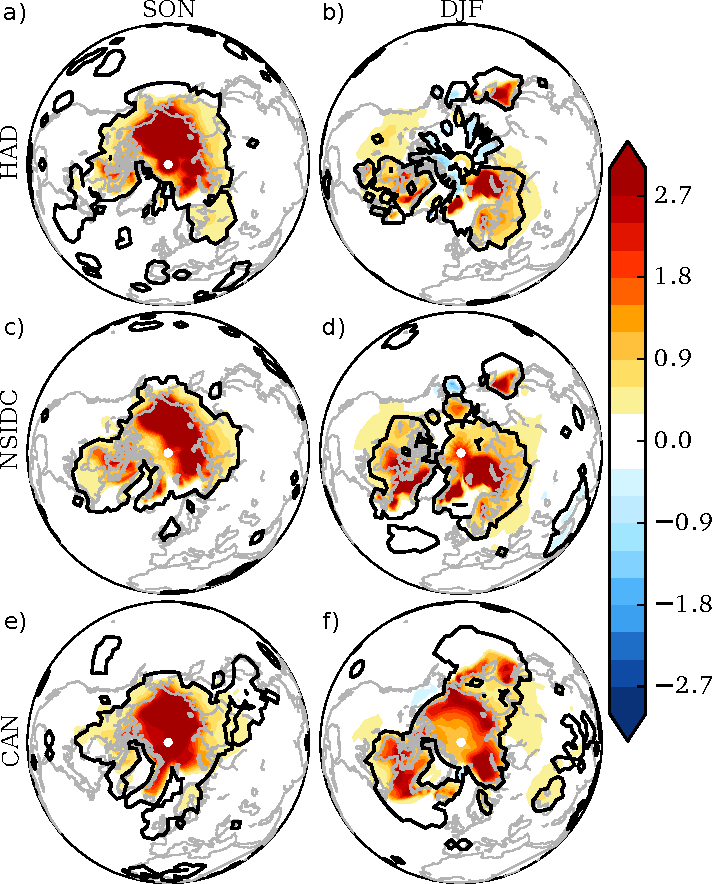
\includegraphics[width=19pc,angle=0]{SATmaps.pdf}\\
  \caption{SAT maps
}\label{fig:fig3}
\end{figure}

\begin{figure}[t]
  \noindent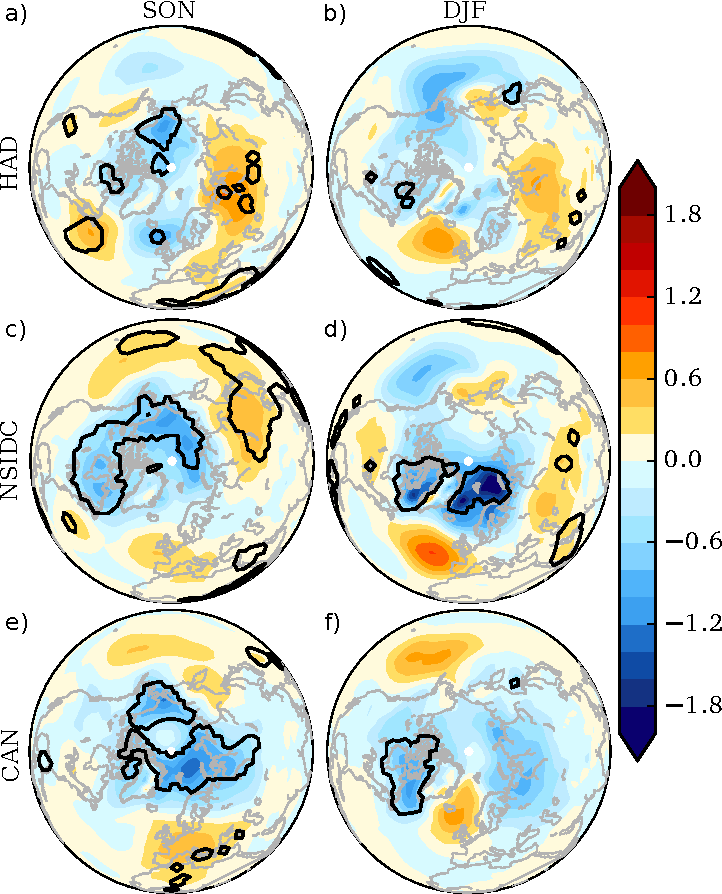
\includegraphics[width=19pc,angle=0]{SLPmaps.pdf}\\
  \caption{SLP maps.
}\label{fig:fig3b}
\end{figure}

\begin{figure}[t]
  \noindent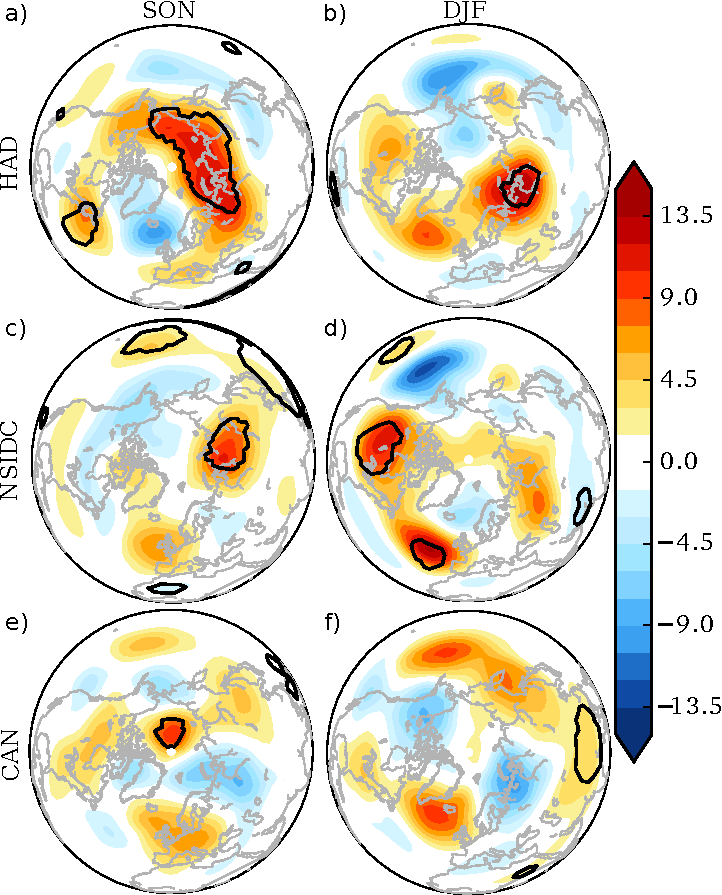
\includegraphics[width=19pc,angle=0]{GZ500maps.pdf}\\
  \caption{Z500 maps.
}\label{fig:fig3c}
\end{figure}

\begin{figure}[t]
  \noindent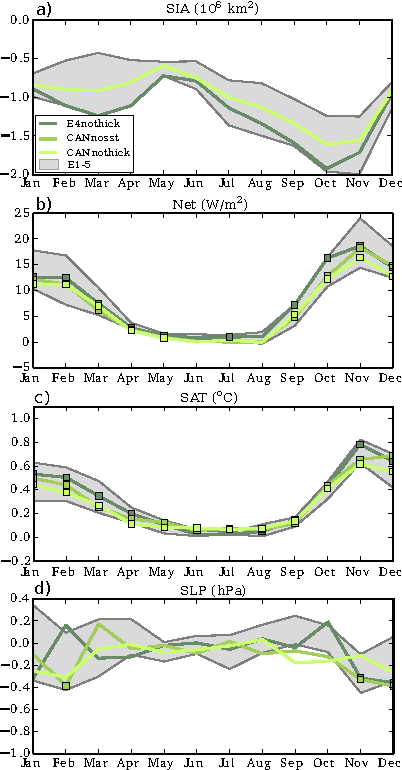
\includegraphics[width=15pc,angle=0]{seacyclessens.pdf}\\
  \caption{As Figure \ref{fig:fig2} but for the sensitivity runs CANE4nosit (dark green), CANnosst (medium green; exactly the same as CANnosit for sea ice area), and CANnosit (light green). 
}\label{fig:fig2b}
\end{figure} % Seasonal cycle of a.) Arctic sea ice area anomaly (10$^6$ km$^2$) for the sensitivity simulations E4nothick (dark green), CANnosst (medium green; exactly the same as CANnosit for sea ice area), and CANnosit (light green). Gray shading indicates the range of sea ice area anomalies in individual ensemble members as in Fig. \ref{fig:fig2}. b.) is as a) but for net surface flux anomaly averaged north of 40$^\circ$N where sea ice concentration $>$ 10\%, c.) is as a) but for surface air temperature anomaly averaged north of 70$^\circ$N, and d.) is as a) but for sea level pressure averaged north of 70$^\circ$N. Squares in b), c), and d) indicate a statistically significant change at the 95\% level using a two-sided student's T test. 

\begin{figure*}[t]
  \noindent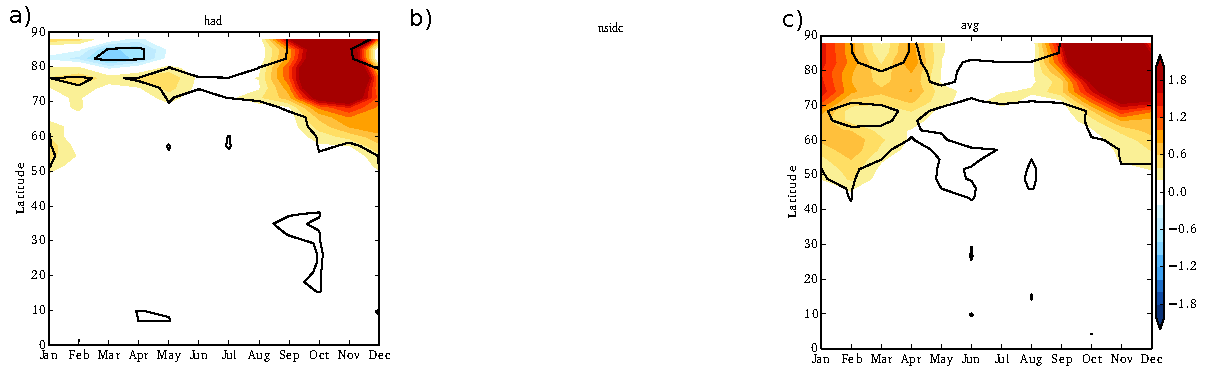
\includegraphics[width=39pc,angle=0]{SATwithlat.pdf}\\
  \caption{Zonal mean surface air temperature anomalies ($^\circ$C) by latitude and month for a.) HAD, b.) NSIDC, and c.) CAN. Black contours indicate statistically significant change at the 95\% level based on a two-sided student's T test. Gray contours show sea ice concentration anomalies for the respective simulations. Sea ice concentration anomalies have been multiplied by -1 for clarity.
}\label{f1b}
\end{figure*}

\begin{figure}
  \noindent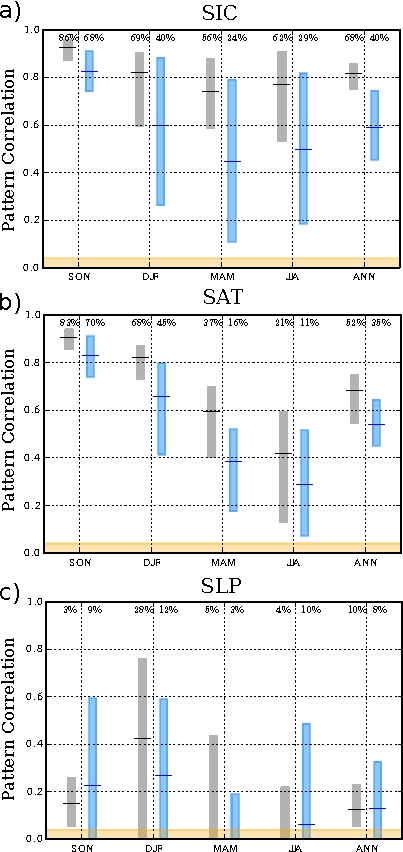
\includegraphics[width=15pc,angle=0]{pattcorrseas_cmpmeanBC.pdf}\\
  \caption{Pattern correlations
}\label{fig:fig4}
\end{figure}

\clearpage

%\begin{figure}[t]
%  \noindent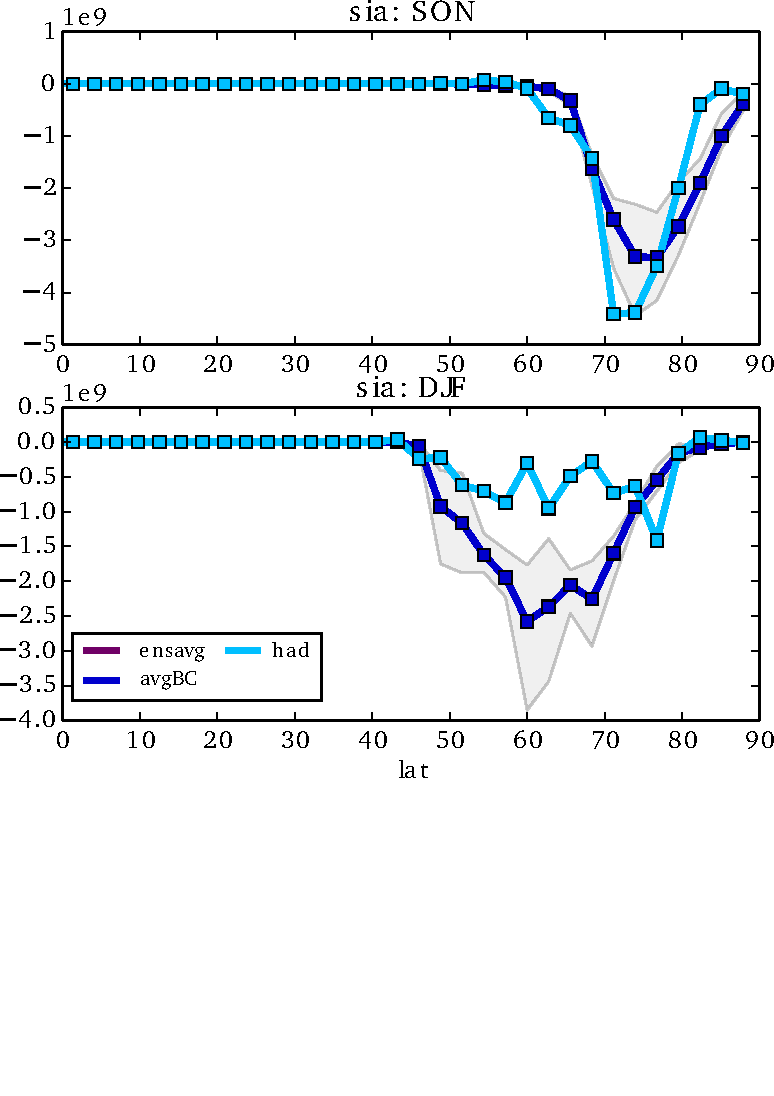
\includegraphics[width=19pc,angle=0]{SIAzonalmean.pdf}\\
%  \caption{Zonal mean sea ice area anomalies ($^\circ$C) with latitude for top) SON, bottom) DJF for the had simulations, avgBC simulations (blue), and the range of e1-5 simulations (gray shading). The mean of the ensemble is by definition the same as the avgBC simulations.
%}\label{f2}
%\end{figure}

%<<<<<<< HEAD
%\begin{figure*}[t]
%  \noindent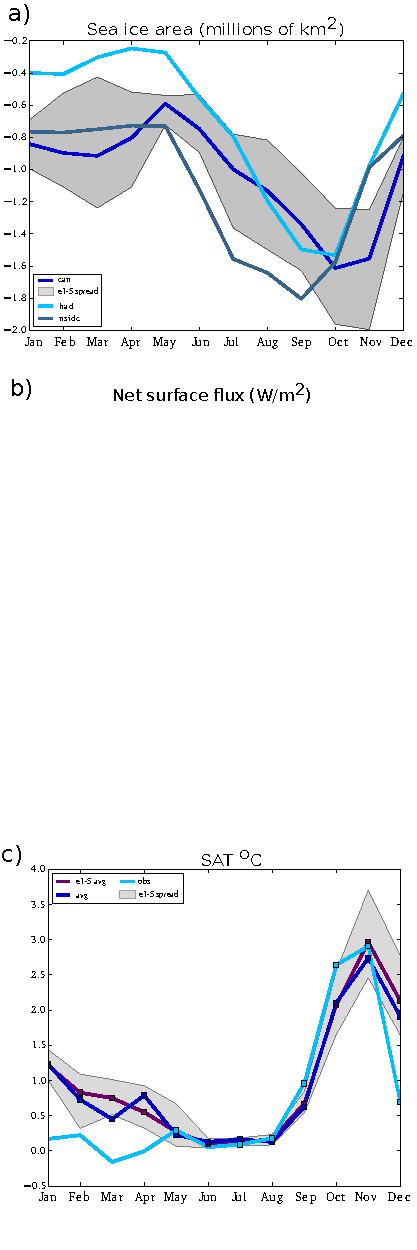
\includegraphics[width=39pc,angle=0]{seacycles.pdf}\\
%  \caption{@@Zonal mean surface air temperature anomalies ($^\circ$C) for a.) PTobs-CTLobs, b.) PTavg-CTLavg. c.) Seasonal cycle of area-averaged SAT North of 70$^\circ$N for all PT simulations and their respective CTL simulations. The gray shading indicates the range of e1-5 ensemble members. Note that here 'obs' indicates the simulations run with boundary conditions derived from observations (HadISST1.1).
%}\label{fig:fig2}
%\end{figure*}
%=======
%
%>>>>>>> FETCH_HEAD

%\begin{figure*}[t]
%  \noindent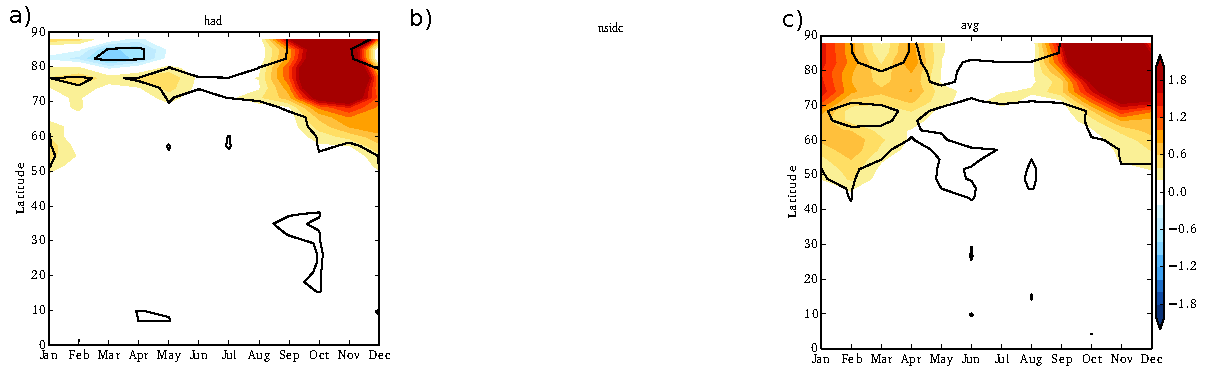
\includegraphics[width=39pc,angle=0]{SATwithlat.pdf}\\
%  \caption{Zonal mean surface air temperature anomalies ($^\circ$C) by latitude and month for a.) hadPT-hadCTL, b.) nsidcPT-nsidcCTL, and c.) canPT-canCTL. Black contours indicate statistically significant change at the 95\% level based on a two-sided student's T test.
%}\label{fig:fig3}
%\end{figure*}


%\begin{figure}[t]
%  \noindent\includegraphics[width=19pc,angle=0]{stdiff_ens_meanBC_allseassp_zonmean_nh2shade.pdf}\\
%  \caption{Zonal mean SAT anomalies ($^\circ$C) with latitude for the had simulations, avgBC simulations (blue), and the range of e1-5 simulations (gray shading). The mean of the ensemble is by definition the same as the avgBC simulations.
%}\label{f3}
%\end{figure}
%
%\begin{figure}[t]
%  \noindent\includegraphics[width=19pc,angle=0]{stdiff_ens_meanBC_r4ct_allseassp_zonmean_nh2.pdf}\\
%  \caption{Zonal mean SAT anomalies ($^\circ$C) with latitude for the had simulations, avgBC simulations (blue), and the range of e1-5 simulations (gray shading). The mean of the ensemble is by definition the same as the avgBC simulations.
%}\label{f4}
%\end{figure}


%%%%%%%%%%%%%%%%%%%%%%%%%%%%%%%%%%%%%%%%%%%%%%%%%%%%%%%%%%%%%%%%%%%%%
% ACKNOWLEDGMENTS
%%%%%%%%%%%%%%%%%%%%%%%%%%%%%%%%%%%%%%%%%%%%%%%%%%%%%%%%%%%%%%%%%%%%%
%
\acknowledgments
Start acknowledgments here.

%%%%%%%%%%%%%%%%%%%%%%%%%%%%%%%%%%%%%%%%%%%%%%%%%%%%%%%%%%%%%%%%%%%%%
% APPENDIXES
%%%%%%%%%%%%%%%%%%%%%%%%%%%%%%%%%%%%%%%%%%%%%%%%%%%%%%%%%%%%%%%%%%%%%
%
% Use \appendix if there is only one appendix.
%\appendix

% Use \appendix[A], \appendix}[B], if you have multiple appendixes.
%\appendix[A]

%% Appendix title is necessary! For appendix title:
%\appendixtitle{}

%%% Appendix section numbering (note, skip \section and begin with \subsection)
% \subsection{First primary heading}

% \subsubsection{First secondary heading}

% \paragraph{First tertiary heading}

%% Important!
%\appendcaption{<appendix letter and number>}{<caption>} 
%must be used for figures and tables in appendixes, e.g.,
%
%\begin{figure}
%\noindent\includegraphics[width=19pc,angle=0]{figure01.pdf}\\
%\appendcaption{A1}{Caption here.}
%\end{figure}

%%%%%%%%%%%%%%%%%%%%%%%%%%%%%%%%%%%%%%%%%%%%%%%%%%%%%%%%%%%%%%%%%%%%%
% REFERENCES
%%%%%%%%%%%%%%%%%%%%%%%%%%%%%%%%%%%%%%%%%%%%%%%%%%%%%%%%%%%%%%%%%%%%%
% Make your BibTeX bibliography by using these commands:
% \bibliographystyle{ametsoc2014}
% \bibliography{references}


%%%%%%%%%%%%%%%%%%%%%%%%%%%%%%%%%%%%%%%%%%%%%%%%%%%%%%%%%%%%%%%%%%%%%
% TABLES
%%%%%%%%%%%%%%%%%%%%%%%%%%%%%%%%%%%%%%%%%%%%%%%%%%%%%%%%%%%%%%%%%%%%%
%% Enter tables at the end of the document, before figures.
%%
%
%\begin{table}[t]
%\caption{This is a sample table caption and table layout.  Enter as many tables as
%  necessary at the end of your manuscript. Table from Lorenz (1963).}\label{t1}
%\begin{center}
%\begin{tabular}{ccccrrcrc}
%\hline\hline
%$N$ & $X$ & $Y$ & $Z$\\
%\hline
% 0000 & 0000 & 0010 & 0000 \\
% 0005 & 0004 & 0012 & 0000 \\
% 0010 & 0009 & 0020 & 0000 \\
% 0015 & 0016 & 0036 & 0002 \\
% 0020 & 0030 & 0066 & 0007 \\
% 0025 & 0054 & 0115 & 0024 \\
%\hline
%\end{tabular}
%\end{center}
%\end{table}

%%%%%%%%%%%%%%%%%%%%%%%%%%%%%%%%%%%%%%%%%%%%%%%%%%%%%%%%%%%%%%%%%%%%%
% FIGURES
%%%%%%%%%%%%%%%%%%%%%%%%%%%%%%%%%%%%%%%%%%%%%%%%%%%%%%%%%%%%%%%%%%%%%
%% Enter figures at the end of the document, after tables.
%%
%
%\begin{figure}[t]
%  \noindent\includegraphics[width=19pc,angle=0]{figure01.pdf}\\
%  \caption{Enter the caption for your figure here.  Repeat as
%  necessary for each of your figures. Figure from \protect\cite{Knutti2008}.}\label{f1}
%\end{figure}

\end{document}